\label{sec:overview}

\begin{figure}[!t]
\begin{center}
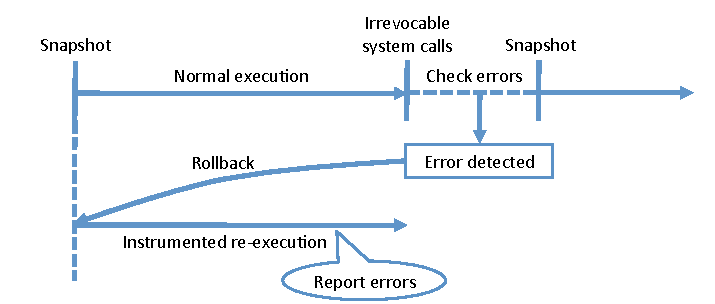
\includegraphics[width=3.3in]{figure/overview}
\end{center}
\caption{
Overview of \doubletake{}: execution is divided into epochs at the boundary of irrevocable system calls. 
\label{fig:overview}}
\end{figure}

\doubletake{} is a high performance dynamic analysis framework for a class of errors that share a \emph{monotonicity} property: evidence of the error is persistent and can be gathered after-the-fact. As Figure~\ref{fig:overview} depicts, program execution is divided into epochs, during which execution proceeds at full speed. At the end of each epoch, marked by irrevocable system calls, \doubletake{} checks program state for evidence of memory errors. If an error is found, the epoch is re-executed with additional instrumentation to pinpoint the exact cause of the error. To demonstrate \doubletake{}'s effectiveness, we have implemented detection tools for heap buffer overflows, use-after-free errors, and memory leaks, which we describe in detail in Section~\ref{sec:applications}.  All detection tools share the following core infrastructure that \doubletake{} provides.

\subsection{Efficient Recording}

At the beginning of every epoch, \doubletake{} saves a snapshot of program registers, and all writable memory. The epoch ends when the program attempts to issue an irrevocable system call, but most system calls do not end the current epoch. \doubletake{} also records the order of thread synchronization operations to support re-execution of parallel programs. \doubletake{} records minimal system state at the beginning of each epoch (like file offsets), which allows system calls that modify this state to be undone if re-execution is required. As a result, most programs require very few epochs and program state checks. We describe the details of each application's state checks in Section~\ref{sec:applications}.

\subsection{Precise Replay}

When program state checks detect an error, \doubletake{} replays the previous epoch to pinpoint the error's root cause. \doubletake{} ensures that all program-visible state, system call results, memory allocations, and the order of all thread synchronization operations are identical to the original run. During replay, \doubletake{} returns saved return values for most system calls, with special handling for some cases. Section~\ref{sec:implementation/normalexecution} describes \doubletake{}'s recording and re-execution of system calls and synchronizations.

\subsection{Custom Heap Allocator}

\doubletake{} replaces the default heap allocator with a new heap built using Heap Layers~\cite{heaplayers}. Detection tools can interpose on heap operations to alter memory allocation requests or defer reuse of freed memory, and can access the heap's map of allocated memory. Memory leak detection uses this map to identify unreachable memory. Buffer overflow and dangling pointer (use-after-free) detection both use heap canaries to detect errors. \doubletake{}'s heap includes a bitmap to track the locations of heap canaries, and automatically checks the state of canaries at the end of each epoch. Section~\ref{sec:heapallocator} presents further details.

\subsection{Watchpoints}

\doubletake{} lets detection tools set hardware watchpoints during re-execution. A small number of watchpoints are available on modern architectures (four on x86). Each watchpoint can be configured to pause program execution when a specific byte or word of memory is accessed. Watchpoints are primarily used by debuggers, but previous approaches have used watchpoints for error detection as well~\cite{Kivati,fastboundschecking}. \doubletake{}'s watchpoints are particularly useful in combination with heap canaries. During re-execution, our buffer overflow and use-after-free detectors place a watchpoint at the location of the overwritten canary to trap the instruction(s) responsible for the error.
